\lhead{\emph{Basic Operation}}

\chapter{AMC Prototype Feedback Control Algorithm and its Simulation}\label{ch:operation}

% In Chapter~\ref{ch:amcP}, the overall system has been described.  Each component of the system was discussed in detail.

% This chapter is about
% \begin{itemize}
%     \item how the system works as a unit to provide magnetic field control.  This includes the algorithm which generates the control and some typical results from its operation.  It also includes the methods used in operating the system, such as methods used in tuning the PI control system.
%     \item simulation methods used to understand system performance, and some basic results from the simulation which are compared with data
%     \item definition of metrics that will be used to quantify further system performance.  These will be applied in Chapter~\ref{ch:quantification} where further results will be presented.
% \end{itemize}



% Much of this work follows the work of others, especially Refs.~\cite{bea,rawlik,lins}.  New work that builds on these results is presented in Chapter~\ref{ch:quantification}.

%This chapter describes the main tool that generates the required currents that should be fed to the coils for compensation.
%The algorithm is based on the control theory and similar to as discussed in Ref. \cite{bea}.

In Chapter~\ref{ch:amcP}, the overall system has been described.  Each component of the system was discussed in detail. This chapter is about how the system works as a unit to provide magnetic field control.  This includes the algorithm which generates the control and some typical results from its operation.  It also includes the methods used in operating the system, such as methods used in tuning the control algorithm for the system. In addition to that, it will cover the simulation methods used to understand the system performance and some basic results from the simulation which are compared with the data. Finally, it will end with the definition of metrics that will be used to further quantify the system performance.  These will be applied in Chapter~\ref{ch:quantification} where more results will be presented. Much of this work follows the work of others, especially Refs.~\cite{bea,rawlik,lins}.  New work that builds on these results is presented in Chapter~\ref{ch:quantification}.

\section{Principle of Operation\label{sec:process}}

% The goal of this Section is to tell the general idea of how the system works, and to introduce the principles of operation.  It also introduces a few of the key issues faced when operating the system.

% \begin{itemize}
%     \item fluxgates (hopefully described in some Section in Chapter~\ref{ch:amcP}) measure the field
%     \item a setpoint for each fluxgate axis is decided
%     \item when the fluxgate signal drifts from the setpoint, the error grows
%     \item how the fluxgates respond to changes in the current is described by a matrix
%     \item the inverse of the matrix describes how to correct the currents based on fluxgate signals
%     \item PI control is used to decide the corrected currents based on the input errors from the fluxgate readings
% \end{itemize}

% Details:
% \begin{itemize}
%     \item the matrix isn't square and its inverse has to be defined
%     \item the problem can be ill-conditioned so that the matrix must be regularized in order that small changes in currents do not generate large, uncontrolled fluctuations in field.  The regularization itself is nontrivial.
%     \item the PI loop must be tuned
% \end{itemize}


% \fig{Images/feedback}{width = 0.6\textwidth}{PI loop in flow chart.\label{fig: feedback}}
% The first measurement from the sensors after filtering (see section \ref{sec:f}) will act as setpoint ($B_{setpoint}$)


% The basic idea is that there will be a goal/setpoint with whom the consecutive measurement will be compared and any deviation from the setpoint will be minimized by the Proportional Integral (PI) feedback algorithm. For this prototype, the first measurement from the sensors after filtering (see section \ref{sec:filter}) will act as setpoint. Then the repeated measurements from the sensors have been taken. For each measurement, difference with the setpoint is  noted as -
% \begin{equation*}
%     \Delta B = B(setpoint) - B(measure)
% \end{equation*}
% % The current is related to magnetic field by- 
% % \begin{equation*}
% %     B=M \times I
% % \end{equation*}
% % Where, $\bm{M}$ is the matrix of proportionality factor in $nT/A$. So, the difference in current can easily be found by -
% % \begin{equation*}
% %     \Delta I=M^{-1} \times \Delta B
% % \end{equation*}
% On the basis of that, PI feedback algorithm will generate the required current that should be fed to the coils to compensate $\Delta B$. After certain period, a perturbation is also applied using an eletro-magnet coil to test how good the system is performing.  The above process is repeated as long as the compensation is running. 

The goal of this Section is to tell the general idea of how the system works, and to introduce the principles of operation.  It also introduces a few of the key issues faced when operating the system. 

First of all , fluxgates (see Section~\ref{sec:sensor}) is used to measure the magnetic field by placing them in different position within the coil cube (see Section~\ref{sec:cube}) and a setpoint for each fluxgate axis is decided after filtering (see Section~\ref{sec:filter}). When the fluxgate signal drifts from the setpoint, the error grows and how the fluxgates respond to changes in the current is described by a matrix. Moreover, to make the errors even more, a perturbation is also applied using an eletro-magnet coil as descibed in Section~\ref{sec:cube} to test how good the system is performing. The inverse of the matrix describes how to correct the currents based on the errors from the consecutive fluxgate signals. Propotional Integral or simply PI control algorithm  is used to decide the corrected currents based on the input errors from the fluxgate readings. As, the matrix isn't square and its inverse has to be defined. The problem arises as the matrix can be ill-conditioned which must be regularized in order that small changes in currents do not generate large, uncontrolled fluctuations in the field.  The regularization itself is nontrivial. After fixing those, the PI control loop must be tuned also.

In the upcoming Sections, the mathematical definitions required to explain system operation will be discussed. Issues encountered in ill-conditioning and regularization including the mathematical principles of regularization will be covered and some basic results of the measurements after tuning the PI parameters will be shown. Simulations and metrics of the system performance are also discussed. Chapter~\ref{ch:quantification} relates to use of these tools to characterize system performance, focusing on the novel aspects of any work.

\section{Matrix of Proportionality Factors}\label{sec:m}
% where subscript indices $s$, $c$ and $n$ has been used to indicate sensors, coil and no. of measurement respectively.

This Section is about the matrix which relates fluxgate readings to coil currents. As previously discussed in Sections~\ref{sec:cube} and~\ref{sec:sensor}, there are total 14 sensors and 7 coils for the prototype. Among them, 12 sensors and 6 coils are used for compensation and others are used for quantification. The matrix relates the currents in the six coils to the magnetic field readings in the 12 sensors. The magnetic field readings change linearly with current, represented by a constant matrix $\bm{M}$.  The matrix is a constant if we ignore hysteresis.  This is generally a good approximation because the magnetic permeability of the nearby magnetic shields is very large.

The relationship between the relative sensor readings and the coil currents is
\begin{equation}\label{eq:B_coils}
    B_s^n(\mathrm{coils})=\sum_{c=1}^{6} M_{sc} I_c^n
\end{equation}
where, $M_{sc}$ are the elements of the matrix $\bm{M}$ and $I_c^n$ is the current set on the coils for a particular measurements where $n$ runs from 0 to N for N being total no. of measurements. The sum is over coils $c$ where $c$ runs from 1 to 6 and the sensor index $s$ runs from 1 to 12. They have been defined in Table~\ref{table:index}. The field $B_s^n(coils)$ refers only to the relative field, in the sense that it is the field generated at sensor $s$ by the coil set. There could be other fields from the environment, which are the fields we seek ultimately to correct and will be discussed in the following Section~\ref{sec:pi}.


\begin{table} [htb!]
    \centering
    \begin{tabular} { |c|c|c|c|c|c|} 
        \hline
        Index & Range & Labels & Definition\\
        \hline\hline
        $c$ & 1-6  & $C_x^\pm$, $C_y^\pm$ and $C_z^\pm$  & Define specific coil \\ 
        \hline
        $S$ & 1-14  & \makecell{1$x$, 1$y$, 1$z$ or \\3$x$, 3$y$, 3$z$ or\\ center-$x$ ... center-$z$ \\ etc.}  & \makecell{Define the $x$, $y$ and $z$ \\of a specific position \\ (Numbering based \\on positions). \\Control sensors used\\ on the center\\ of the prototype} \\ 
        \hline
        $s$ & 1-12  & \makecell{Same as labels of $S$}  & \makecell{Subset of $S$ excluding\\ the 2 control sensors} \\ 
        \hline
        $n$ &  0$<$N$<\infty$ & 1,2,3,..,N  & \makecell{Define no. of \\PI loop iteration} \\ 
        \hline        
    \end{tabular}
    % \vspace{4mm}
    \caption[Definition of different indices to indicate sensor, coil and no. of iteration in the feedback loop]{Definition of different indices to indicate sensor, coil and no. of iteration in the feedback loop where $s$ or $S$ (if control sensors are included) can be taken different labels based on how the sensor position has been specified. For example- it could start with center-$x$ or 3$x$ which means the first sensor is at position center or 3 as specified in Section~ \ref{sec:cube} in $x$-axis respectively. Similarly, $c$ started with $C_x^-$ means the first coil is $C_x^-$ as defined again in Section~ \ref{sec:cube}. The index $n$ denotes the iteration number of the PI feedback control algorithm. }\label{table:index}
\end{table}

\FloatBarrier


The matrix defined in this way is easy to measure using the system.  Each coil $c$ is set to a current, with all other currents set to zero.  The change in the sensor reading $s$ then gives the matrix element $M_{sc}$. 


\fig{Images/Mdiff3_31}{width = \textwidth}{Color map of $\bm{M}$ measured using the scheme indicated in the text.  Horizontal axis indicates the various sensors, which are counted using the index $s$.  Vertical axis indicates the various coils, which are counted using the index $c$.  The color axis ($z$-axis) indicates the value of the matrix element.  Red elements indicate positive values while blue elements indicate negative values.  Elements that appear white are near zero in the matrix element.\label{fig:m}}{Color map of $\bm{M}$}

\FloatBarrier
The color map of a matrix $\bm{M}$ measured in this fashion is shown in Fig.~\ref{fig:m}.  The results are reasonable considering the design of the system.  The system was designed to compensate magnetic field of order 100~nT for currents of 200~mA, which would imply the matrix elements should be of scale 500~nT/A.  Generally this agrees with the color scale seen in Fig.~\ref{fig:m}.  Furthermore, the strongest matrix elements are those where the coil is closest to the sensor in question.  For example, 8y is closest to coils Y- and X+.  It also makes sense that 8y would have strong matrix elements here because it is near the corner of the magnetic shield which causes {\it e.g.} the X+ coil to be converted into a strong y component.  The red and blue colors are a result of the definitions of positive/negative current in relation to coil in question's orientation and the sensor axis definition.



\section{Implementation of PI Control Algorithm}\label{sec:pi}
 In my algorithm, the magnetic field is measured using the fluxgates and used to define the setpoints. As will be shown, when the field changes, the error in the field can be translated into an error in current based on inverting Eq.~(\ref{eq:B_coils}). New current values are then calculated that must be fed to the coils completing the PI control loop. 

% The measurement from the fluxgate sensors will have  the contribution from both the environment and  the field generated at sensors by the coil set of specific current value as presented in Eq.~(\ref{eq:B_coils} and can be related by 
% \begin{equation}\label{eq:B}
%     B_s^n (measure) = B_s^n(environment)+ B_s^n(coils)
% \end{equation}

The typical magnetic field of the surroundings has been measured using a fluxgate and is reported in Table~\ref{table:Benvironment}. The values are similar in scale to Earth$'$s magnetic field which is $\sim$45 $\mu$T in vertical downward direction. These are the typical scale of the setpoints.

\begin{table} [htb!]
    \centering
    \begin{tabular} { |c|c|c|c|c|c|} 
        \hline
        Axis & \makecell{Typical B field \\($\mu$ T)}\\
        \hline\hline
        $x$ & 10 \\ 
        \hline
        $y$ & 42 \\ 
        \hline
        $z$ & -5 \\ 
        \hline
    \end{tabular}
    % \vspace{4mm}
    \caption[Typical magnetic fields surrounding the prototype]{Typical magnetic field values of the environment surrounding the prototype obtained from fluxgate measurements when the $x$, $y$ and $z$ axis represent the northward, vertical downward, and westward direction respectively. }\label{table:Benvironment}
\end{table}

\FloatBarrier
For PI control, the setpoint is measured using the fluxgate array by applying 100 mA current to the coils. Our current sink (see Section~\ref{sec:sink}) can generate 0-200 mA current. So, the 100 mA current has been chosen to utilize the full capacity of the current sink to compensate the field fluctuations in either direction. After finding the setpoint from the first measurement of the fluxgates, the change in the fluxgate signal is
\begin{equation}\label{eq:del_B}
    \Delta B_s^n = B_s(setpoint) - B_s^n(measure)
\end{equation}

For iteration $n=1$, Eq~(\ref{eq:del_B}) will give zero value as the first measurement is acting as to be setpoint, as explained earlier. The consecutive measurements are used in the control algorithm. 

Using the relationship between the sensor readings and the coil currents as explained in Eq.~(\ref{eq:B_coils}) and the $\Delta B_s^n$ obtained from Eq.~(\ref{eq:del_B}), the error in terms of the current  will be
\begin{equation}\label{eq:del_I}
    \Delta I_c^n =\sum_{s=1}^{12} M^{-1}_{cs} \Delta B_s^n
\end{equation}
Here, $M^{-1}_{cs}$ are the elements of the inverse of the matrix $\bm{M}$. The inversion of the non-square matrix is a subtle problem and is discussed in Section~\ref{sec:inv}. The sum in Eq.~(\ref{eq:del_I}) is over sensors $s$ and the coil index $c$ runs from 1 to 6 as defined in Table~\ref{table:index}. $\Delta I_c^n$ is the error for $n^{\mathrm{th}}$ measurement on the basis of which the new set of currents will be calculated using a PI control algorithm. In the algorithm, the new current~\cite{bea} is
\begin{equation}\label{eq:I}
    I^n_c=I^0_c+k^p_c \Delta I_c^n+k^i_c\sum_n \Delta I_c^n
\end{equation}
where, $I^0_c$ indicates the initial value of current for the set of the coils when the setpoint has been set (100 mA). $\Delta I_c^n$ is the error found using Eq.~(\ref{eq:del_I}) and the sum is over no. of iterations $n$ where $n$ runs from 1 to $N$ as explained in Table~\ref{table:index}. The term $k^p_c$ is the proportional gain (P) and $k^i_c$ is the integral reset (I) for a particular coil. P and I that is $k^p_c$ and $k^i_c$ terms need to tune properly before they calculate the new current which will be explained later in Section~\ref{sec:tune}. The index $c$ in $k^p_c$ and $k^i_c$ terms represent the P and I value for coils $c$ where $c$ runs from 1 to 6. But throughout the thesis, I have used same values of $k_c^p$ and $k_c^i$ in all six coils. As only P and I terms have been used, so it is called Proportional Integral or simply PI controller~\cite{pid}. We limit ourselves from using derivative term (D) because of the amplification of noise while using it.

\fig{Images/1s1c1zc1}{width = \textwidth}{The $C_x^-$ coil current (left) and magnetic field $\Delta B$ (right) for sensor 1z with $k_c^p=1.0$, and $k_c^i=0.0$. Green curve:  measured field change $\Delta B$.  Red curve: predicted uncompensated field change. Vertical dashed lines indicate the time of the perturbation coil being turned on and off.\label{fig:1s1c1zc1} }{The compensation effect on single sensor due to single coil.}

Fig.~\ref{fig:1s1c1zc1} shows a simple one dimensional control example implementing PI control algorithm. It is seen that the magnetic field change on sensor position 1z  has been compensated successfully due to coil current $C_x^-$. 


Next, the inversion process of matrix $\bm{M}$ will be discussed for multidimensional control.


\section{Inversion of Matrix}\label{sec:inv}

This Section describes in detail the inversion process of the non-square matrix $\bm{M}$ and issues encountered. It also discusses the solution to inversion which uses regularization by random fluctuations, a strategy pursued previously by other groups. 


We have a non-square matrix $\bm{M}$ with dimension $6*12$ (coils~$\times$~sensors). The matrix $\bm{M}$ is discussed earlier in Section~\ref{sec:m} and shown in Fig.~\ref{fig:m}. $\bm{M}$ needs to be inverted for calculating the error using Eq.~\ref{eq:del_I}.
% \fig{Images/1s2c3zc1c62}{width = \textwidth}{The compensation effect on sensor position 1z due to coil $C_x^-$ and coil $C_z^+$. Vertical axis in left shows the coil currents that have been sent to coils $C_x^-$ (blue color) and $C_z^+$ (green color). $C_x^-$ and $C_z^+$ have been separated by 40 mA for showing them together in the same figure. Vertical axis in right shows the $\Delta$ B found using Eq.~(\ref{eq:del_B}), where the blue color indicates $\Delta$ B due to compensation and the red indicates $\Delta$ B without compensation. In both figures, the red color dashed line indicates the time when the perturbation coil is turned on and the green color dashed line indicates when that is turned off. For position of the sensor and coils see the Fig.~\ref{fig:coil}.\label{fig:1s2c3zc1c6}}{The compensation effect on single sensor due to two coils.}


% Similar effect has been found if we use two coils current to control one sensor as shown in Fig.~\ref{fig:1s2c3zc1c6}. It is seen that the magnetic field on sensor position 1z (right) due to coils current $C_x^-$ and $C_z^+$ (left) has been stablized very well indicated by the blue color (right) as compared to the field that would have been without compensation indicated by the red color. 

% \fig{Images/2s1c3y3zc12}{width = \textwidth}{The compensation effect on sensor position 1y and 1z due to coil $C_x^-$. Vertical axis in left shows the coil currents that have been sent to coil $C_x^-$. Vertical axes in middle and right show the $\Delta$ B found using Eq.~(\ref{eq:del_B}), where the blue (middle) and green (right) colors indicate $\Delta$ B due to compensation and the red in both indicates $\Delta$ B without compensation. In all three figures, the red color dashed line indicates the time when the perturbation coil is turned on and the green color dashed line indicates when that is turned off. For position of the sensors and coil see the Fig.~\ref{fig:coil}.\label{fig:2s1c3y3zc1}}{The compensation effect on two sensors due to one coils.}


% We have also tested the magnetic compensation effect on two sensor positions due to single coil current as shown in Fig.~\ref{fig:2s1c3y3zc1}. It is seen that the magnetic field fluctuations ($\Delta$ B found using Eq.~(\ref{eq:del_B})) on sensor positions 1y (middle) and 1z (right) due to coil current $C_x^-$ (left) are similar/more while compensation indicated by blue color (middle) and green color (right) as compared to without compensation indicated by the red color. So, if we don$'$t have a matrix to deal with, this system seems to work fine.














% \begin{figure}[!htb]
%     \begin{subfigure}{.5\linewidth}
%         \centering
%         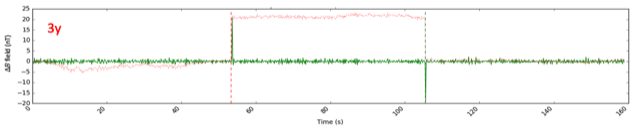
\includegraphics[width=\linewidth, height= 3 cm]{Images/1s1c3y}
%         \caption{for 3y and $C_x^-$ }
%         \label{fig:1s1c3y}
%     \end{subfigure}%
%     \begin{subfigure}{.5\linewidth}
%         \centering
%         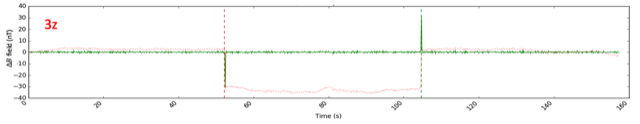
\includegraphics[width=\linewidth, height= 3 cm]{Images/1s1c3z}
%         \caption{for 3z and $C_x^-$}
%         \label{fig:1s1c3z}
%     \end{subfigure}\\[1ex]
%     \begin{subfigure}{.5\linewidth}
%         \centering
%         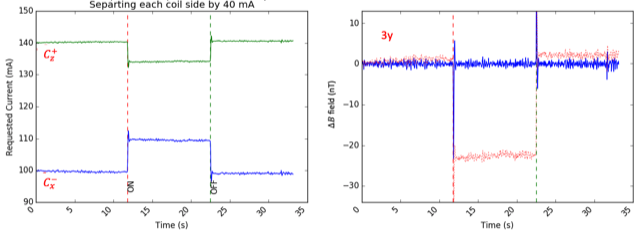
\includegraphics[width=\linewidth, height= 3 cm]{Images/1s2c3yc1c6}
%         \caption{for 3y, 3z, $C_x^-$ and $C_z^+$}
%         \label{fig:1s2c3yc1c6}
%     \end{subfigure}%
%         \begin{subfigure}{.5\linewidth}
%         \centering
%         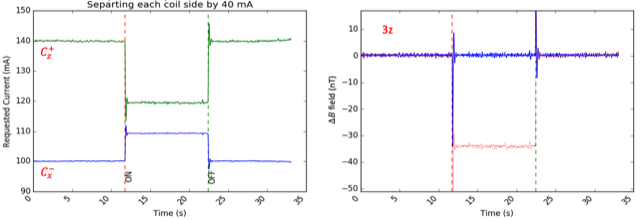
\includegraphics[width=\linewidth, height= 3 cm]{Images/1s2c3zc1c6}
%         \caption{for 3y, 3z, $C_x^-$ and $C_z^+$}
%         \label{fig:1s2c3zc1c6}
%     \end{subfigure}\\[1ex]
%     \begin{subfigure}{1\linewidth}
%         \centering
%         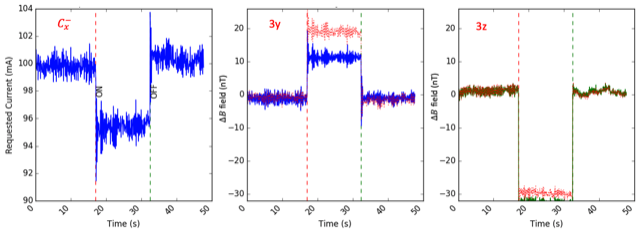
\includegraphics[width=\linewidth, height= 3 cm]{Images/2s1c3y3zc1}
%         \caption{for 3y, 3z and $C_x^-$ }
%         \label{fig:2s1c3y3zc1}
%     \end{subfigure}

%     \caption{The compensation effect due to individual coil. Vertical axis in Fig.~\ref{fig:1s1c3y} and in Fig~\ref{fig:1s1c3z} shows the $\Delta$ B found using Eq.~\ref{eq:del_B} over time for two different sensors where the green indicates $\Delta$ B due to compensation and the red indicates $\Delta$ B without compensation. Vertical axis in left of both Fig.~\ref{fig:1s2c3yc1c6} and  Fig.~\ref{fig:1s2c3zc1c6} indicates the coil current that has been sent to coils $C_x^-$ and $C_z^+$ to satblize 3y and 3z as shoen in right of those respectively. Initially both $C_x^-$ and $C_z^+$ were in the same level but for showing them together in the same figure they have been separated by some constant.  Vertical axis in left of Fig.~\ref{fig:2s1c3y3zc1} also indicates the current but only for $C_x^-$. Vertical axis in right of Fig.~\ref{fig:1s2c3yc1c6} and  Fig.~\ref{fig:1s2c3zc1c6} and in middle and right of Fig.~\ref{fig:2s1c3y3zc1} have the same description as in in Fig~\ref{fig:1s1c3z} }
%     \label{fig:1d}
% \end{figure}

% \FloatBarrier
% The author in Ref.~\cite{bea} in Section \textcolor{blue}{7.2.3} of her PhD thesis claimed that more sensors than coils with some optimization give better compensation forming a non-square matrix which needs to be inverted for calculating the error using Eq.~\ref{eq:del_I}. 

The Moore--Penrose pseudoinverse can be used for the inversion process. A tutorial review of the pseudoinverse can be found in Ref.~\cite{pseudo}. The pseudoinverse of a matrix can be computed using singular value decompostion (SVD). SVD is a factorization or diagonalization of a matrix. The matrix can be real or complex square or rectangular matrix. The SVD~\cite{svd2,svd3} of a real rectangular matrix $\bm{M}$ with dimension $s \times c$ and $s>c$ is 
\begin{equation}\label{eq:m}
        \bm{M} = \bm{U} \bm{\Sigma} \bm{V^T}
\end{equation}
% where, $\bm{U}\:\epsilon\:\mathbb{R}^{m \times m}$, $\bm{V^*}\:\epsilon\:\mathbb{R}^{n \times n}$ 
where, $\bm{U}$ and $\bm{V}$ are the orthogonal matrices with dimensions $s \times s$ and $c \times c$ respectively and $\bm{V^T}$ is the transpose of $\bm{V}$. $\bm{\Sigma}$ is a real non-negative diagonal matrix with same dimension as  $\bm{M}$ and can be written as

\begin{equation*}
\bm{\Sigma} = \begin{pmatrix} 
\Sigma_{11} &  &  & 0 \\
  & . &  &  \\
  &   & . &  \\

0 &  &  & \Sigma_{nn} \\
 \end{pmatrix}
\end{equation*}
where, $\Sigma_{11},..,\Sigma_{nn}=\sigma_{n}$ are diagonal values of $\bm{\Sigma}$ with $\Sigma_{11}\gg... \Sigma_{nn}\geq0$. The positive square roots of the non-negative eigenvalues of $\bm{M^T}\bm{M}$ yield $\sigma_{n}$, and are called singular values of $\bm{M}$. 

The point of SVD is that this is easy to invert because the transpose of an orthogonal matrix is equal to its invert. That is   $\bm{U^T}=\bm{U^{-1}}$ and $\bm{V^T}=\bm{V^{-1}}$ and
\begin{equation}\label{eq:sigma_inv}
\frac{1}{\bm{\Sigma}} = \begin{pmatrix} 
\frac{1}{\Sigma_{11}} &  &  & 0 \\
  & . &  &  \\
  &   & . &  \\

0 &  &  & \frac{1}{\Sigma_{nn}} \\
 \end{pmatrix}
\end{equation}

The pseudoinverse of $\bm{M}$ will be then the inverse of $\bm{U}$, $\bm{\Sigma}$ and $\bm{V^T}$ and can be written as
\begin{equation}\label{eq:psMinv}
    \bm{M^{-1}} = \bm{V \Sigma^{-1} U^T}
\end{equation}


% ${\rm I\!R}$
%  \fig{Images/6c_U_Mcond26_p1368}{width = \textwidth}{Color map of $\bm{U}$ for transpose of $\bm{M}$ shown in Fig.~\ref{fig:m}. $\bm{U}$ is orthonormal eigenvectors of $\bm{M}\bm{M^T}$ in sensors$\times$sensors dimension for 12 sensors signals (nT). Red elements indicate positive values while blue elements indicate near zero values. \label{fig:6c_U}}{Color map of $\bm{U}$.}

 \fig{Images/V_30}{width = \textwidth}{Color map of $\bm{\Sigma}$ for transpose of $\bm{M}$ shown in Fig.~\ref{fig:m}. $\bm{\Sigma}$ is positive square roots of the non-negative eigenvalues of $\bm{M^T}\bm{M}$ in sensors$\times$coils dimension for 12 sensors and 6 coils in nT/A. Red elements indicate positive values while blue elements indicate near zero values. \label{fig:v}}{Color map of $\bm{\Sigma}$}

%  \fig{Images/6c_Wt_Mcond26_p1368}{width = \textwidth}{Color map of $\bm{V^T}$ for transpose of $\bm{M}$ shown in Fig.~\ref{fig:m}. $\bm{V^T}$ is orthonormal eigenvectors of $\bm{M^T}\bm{M}$ in coils$\times$coils dimension for 6 coils currents (A). Red elements indicate positive values while blue elements indicate near zero values. \label{fig:6c_Vt}}{Color map of $\bm{V^T}$.}

% In earlier Section we have discussed a matrix $\bm{M}$ which is shown in Fig.~\ref{fig:m}. $\bm{M^T}$ is the transpose of that matrix. $\bm{M^T}$ has been decomposed via SVD in $\bm{U}$ , $\bm{\Sigma}$ and $\bm{V^T}$ which are shown in Fig.~\ref{fig:6c_U}, Fig.~\ref{fig:v} and Fig.~\ref{fig:6c_Vt} respectively. The $\bm{\Sigma}$ in Fig.~\ref{fig:v} shows that except diagonal values all are zero with the diagonal values are arranged from $\Sigma_{11}$ to $\Sigma_{nn}$ in a decreasing order each having non-negative values. 

% From those values the condition number of $\bm{M^T}$  can be found. The condition number of a matrix measures the change in the output for a small change in input. Large condition number indicates ill-conditioned matrix while small condition number indicates well-conditioned matrix. The condition number of $\bm{M^T}$ can be determined from the diagonal matrix $\bm{\Sigma}$ as 
%  \begin{equation}\label{eq:cond}
%      cond(\bm{M})=\frac{max(\sigma_n)}{min(\sigma_n)}
%  \end{equation}
 
% Using Eq.~(\ref{eq:cond}), the condition number of $\bm{M^T}$=5676/215=26.4 which indicates an ill-conditioned matrix.

But I found that matrix $\bm{M}$ has some small singular values {\it e.g} small $\sigma_n$. The diagonal elements $\sigma_n$ of $\bm{\Sigma}$ represent eigenvalues. Since no. of coils ($c$) is less than no. of fluxgate sensors ($s$), it is easily thought of as represent modes of the coil set. A large $\Sigma_{11}$ represents a coil mode where a small change in current gives rise to a large change in field. If $\Sigma_{nn}<<\Sigma_{11}$ it means that mode corresponding to  $\Sigma_{nn}$ requires a much larger current in order to generate the same scale of magnetic field as for the $\Sigma_{11}$ mode. 

\begin{equation}\label{eq:del_I_pseudo}
    \Vec{\Delta I} \approx\bm{M^{-1}}\Vec{\Delta B}=\bm{V \Sigma^{-1} U^T}\Vec{\Delta B}=\sum_{n=1}^{rank(\bm{M})}\frac{v_n u_n^T \Vec{\Delta B}}{ \sigma_n}
\end{equation}

It is seen that $\Vec{\Delta I}$ is dominated by the singular vectors $v_n$ due to small $\sigma_n$.

% The condition number of $\bm{M}$ being large therefore indicates that problematic modes exist which will have practically no control on the magnetic field.
In Section~\ref{sec:coil_config} we analyzed this effect further in both simulation and experiment. 
For now, we present the strategy of Ref.~\cite{bea} which we followed initially and it involved regularization.

 
Regularization methods help to reduce the dominance $v_n$. Tikhonov regularization~\cite{tikhonov2013numerical,tikhonov_book,svd,svd3} is one of the most commonly used regularization methods which solves the problem as 

\begin{equation}
    ||\Vec{\Delta B}-\bm{M}\Vec{\Delta I}||_2^2+{\alpha}^2||\Vec{\Delta I}||_2^2
\end{equation}


which modifies the diagonal elements of $\Sigma^{-1}$ from Eq.~(\ref{eq:psMinv}) as

\begin{equation}\label{eq:minvR}
    \frac{1}{\sigma_n} \rightarrow \frac{\sigma_n}{\sigma_n^2+\alpha^2} 
\end{equation}
Tikhonov regularization has been further modified by defining $\alpha=10^r$ as in the previous study \cite{bea}) where, $r$ is called the regularization parameter. If  $r \rightarrow - \infty$, Eq.~(\ref{eq:minvR}) becomes the same as Eq.~(\ref{eq:sigma_inv}) hence no regularization whereas $r \rightarrow + \infty$ results in $\bm{M^{-1}} \rightarrow 0$ i.e. no control. Generally, $r$ should be of order $\mathbf{log}(\sigma_{d})$ in order for regularization to have its desired effect of making the diagonal values of $\bm{\Sigma^{-1}}$ more equal. Example : suppose $\sigma_1$=100 and $\sigma_n$=1 and $\alpha$=10.

\begin{equation*}
    \frac{1}{\sigma_1} \rightarrow \frac{100}{100^2+10^2}=\frac{1}{101} 
\end{equation*}
\begin{equation*}
    \frac{1}{\sigma_n} \rightarrow \frac{1}{1^2+10^2}=\frac{1}{101} 
\end{equation*}
Therefore, the singular values become equalized.

The value of $r$ may be selected using several iterative methods. The obtained $r$ can be directly used in feedback algorithm to determine $\bm{M^{-1}}$. Because, $\bm{M^{-1}}$ appears in the definition of the error in current (Eq.~(\ref{eq:del_I})). It has an effect also on the PI parameters. The PI parameters can be tuned in concept with $r$ by observing the effect on current response and this was studied further in Section~\ref{sec:r_pi}.


An iterative method has been discussed in  the previous study~\cite{bea} to find $r$. The concept has been applied to the prototype which will be discussed next.

% \FloatBarrier

% \begin{equation}\label{eq:sigma}
%     \frac{1}{\sigma_d} \rightarrow \frac{\sigma_d}{\sigma_d^2+(10^r)^2}
% \end{equation}

% So, the Eq.~(\ref{eq:psMinv}) will be modified due to the modified form of Tikhnov regularization as
% \begin{equation}\label{eq:minvR}
%     \bm{M^{-1}}(r) = \bm{V}\begin{pmatrix} 
% \frac{\sigma_1}{\sigma_1^2+(10^r)^2} & 0 \\
% 0 & \frac{\sigma_d}{\sigma_d^2+(10^r)^2}
% \end{pmatrix} \bm{U^T}
% \end{equation}



% \fig{Images/v}{width = \textwidth}{Color map of $\Sigma$ for a test $\bm{M}$ found using Python programming language. Horizontal axis indicates the various coils, which are counted using the index $c$. Vertical axis indicates the various sensors, which are counted using the index $s$. Red elements indicate positive values while blue elements indicate near zero values. \label{fig:v}}{Color map of $\Sigma$}

% \FloatBarrier

% The problem can visualized from Fig.~\ref{fig:m} where for example X-(1) has negligible sensitivity for 3x which means that particular matrix element (in nT/A) is very small. So, the pseudoinverse of $\bm{M}$ using Eq.~\ref{eq:psMinv} will produce very large element (in A/nT) which means that the amount of current will be huge there which will make the prototype unstable. To minimize the effect, the matrix must be regularized which means that all ill-conditioned places must be replaced  by well-conditioned ones.  



\subsection{Regularization by Random Fluctuation}\label{sec:mont}

The method of a previous study~\cite{bea} was reproduced for my prototype to determine a value of $r$ by study its effect on the ability to cancel random field fluctuations without generating unacceptably large current fluctuations.

For the method, a different sets of reasonable random magnetic fields ($B_s^{\text{rand}}$) are generated according to the normal distribution with a central value of 0 and standard deviation 1.5 nT. As in Ref.~\cite{bea}, the reasonable value for the standard deviation was determined by the scale of the fluctuations seen from second to second by the sensor array. The exact value of the standard deviation will turn out to be unimportant in the way Ref.~\cite{bea} finally deduces $r$ using normalized field and current fluctuations.

Using the setpoint as zero, according to Eq.~(\ref{eq:del_B}) the change in the B field is  
\begin{equation}\label{eq:del_Bs}
    \Delta B_s^{\text{sim}} = 0 - B_s^{\text{rand}}=-B_s^{\text{rand}}
\end{equation}

The array of the current errors  as function of $r$ due to the the change in field $\Delta B_s^{\text{sim}}$ is then calculated using the regularized pseudoinverse using Eq.~(\ref{eq:del_I}) as
\begin{equation}\label{eq:del_Is}
    \Delta I_c^{\text{sim}}(r) =\sum_{s=1}^{12} M^{-1}_{cs}(r) \Delta B_s^{\text{sim}}=\sum_{s=1}^{12} M^{-1}_{cs}(r) (-B_s^{\text{rand}})
\end{equation}

To estimate the overall response from the array of the current, the root mean square (RMS) of $\Delta I_c^{\text{sim}}(r)$ is calculated as
\begin{equation}\label{eq:delta_Isim_rms}
     \Delta I_{\text{RMS}}^{\text{sim}}(r)= \sqrt{\frac{1}{6}\sum_{c=1}^6 (\Delta I_c^{\text{sim}}(r))^2}
\end{equation}

Since, $\Delta I_c^{\text{sim}}(r)$ depends on both $r$ and $B_s^{\text{rand}}$, $ \Delta I_{\text{RMS}}^{\text{sim}}(r)$  is calculated as a function of $r$ for different sets of $B_s^{\text{rand}}$ (Fig.~\ref{fig:Isim}). It is noticeable that with the increase of $r$, the current fluctuations $\Delta I_{\text{RMS}}^{\text{sim}}$ vanish as expected.


% $ \Delta I_{\text{RMS}}^{\text{sim}}(r)$ as indicated by vertical axis over $r$ as indicated by horizontal axis has been shown for 30 different sets of $B_s^{\text{rand}}$. The distribution $B_s^{\text{rand}}$ is randomly chosen with center of distribution and standard deviation is discussed earlier. 

\fig{Images/6c_I}{width = \textwidth,height =9.5cm}{The effect of $r$ on the coil currents for 30 different sets of $B_s^{\text{rand}}$ generated according to the normal distribution with a central value of 0 and standard deviation 1.5 nT. The horizontal axis represents $r$ while the vertical axis shows $\Delta I_{\text{RMS}}^{\text{sim}}$. \label{fig:Isim}}{The effect of $r$ on the coil currents.}

\FloatBarrier
The field produced by $ \Delta I_c^{\text{sim}}$ can be calculated using Eq.~(\ref{eq:B_coils}). Thus the total field at each sensor $s$ will be the superposition of $B_s^{\text{rand}}$ and the response produced by $ \Delta I_c^{\text{sim}}(r)$ 
\begin{equation}\label{eq:B_coils-sim}
    B_s^{\text{sim}}(r) =\sum_{c=1}^6 M_{sc} \Delta I_c^{\text{sim}}(r) + B_s^{\text{rand}}
\end{equation}
For a perfectly compensated system, the field produced by $ \Delta I_c^{\text{sim}}$ would equal $- B_s^{\text{rand}}$ which in turn would make the $B_s^{\text{sim}}(r)$ in Eq.~(\ref{eq:B_coils-sim}) identically zero. In practise, this is rarely the case. To quantify the effectiveness of the compensation,  the ratio of RMS of $B_s^{\text{sim}}(r)$ to the RMS of $B_s^{\text{rand}}$ is calculated as
\begin{equation}\label{eq:fluc}
    F(r)=\frac{\sqrt{\frac{1}{12} \sum_{s=1}^{12} (B_s^{\text{sim}}(r))^2}}{\sqrt{\frac{1}{12} \sum_{s=1}^{12} (B_s^{\text{rand}}(r))^2}}
\end{equation}
The function $F(r)$ would be zero for a perfectly compensated system and unity for an uncompensated system. In Ref.~\cite{bea}, $F(r)$ is called the "remaining noise". The values of $F(r)$ is shown in Fig.~\ref{fig:fluc-sim} for same sets of $B_s^{\text{rand}}$ used in Fig.~\ref{fig:Isim}. It is seen that with the increase of $r$, the field produced due to $\Delta I_c^{\text{sim}}$ to compensate $B_s^{\text{rand}}$  are increasing i.e. more field fluctuations. It is also noticeable that the system can not be fully compensated due to the field produced by $ \Delta I_c^{\text{sim}}(r)$ as $F(r)$ never goes to zero. The lowest $F(r)$ is 0.45, indicating the system will not be terribly successful at correcting random fluctuations. We think this is mainly due to the purposely limited design used for this prototype, which was designed instead to focus on issues in multi-dimensional PI control.

\fig{Images/6c_f}{width = \textwidth,height =9.5cm}{The effect of $r$ on horizontal axis on the compensation due to the field produced by $ \Delta I_c^{\text{sim}}(r)$ to counteract $B_s^{\text{rand}}$ indicated by $F(r)$ on vertical axis. The different curves indicate 30 different sets of $B_s^{\text{rand}}$ with the distribution describes earlier. \label{fig:fluc-sim}}{The effect of $r$ on remaining fluctuations.}

\FloatBarrier
It is seen from the Fig.~\ref{fig:Isim} and Fig.~\ref{fig:fluc-sim} that with the increase of $r$, current fluctuations are decreasing but field fluctuations are increasing step. Ref.~\cite{bea} suggested a compromise between them be struck to determine the value of $r$, $\it i.e.$ that reducing current fluctuations ($r \rightarrow + \infty$) be traded off against reducing magnetic field fluctuations ($r \rightarrow - \infty$). to decide the value of $r$, $\Delta I_{\text{RMS}}^{\text{sim}}(r)$ and $F(r)$ were normalized as

\begin{equation}\label{eq:Inorm}
    \overline{\Delta I_{\text{RMS}}^{\text{sim}}}(r)=\frac{\Delta I_{\text{RMS}}^{\text{sim}}(r)}{\Delta I_{\text{RMS}}^{\text{sim}}(r\rightarrow - \infty)} \;\mathbf{,\;and}
\end{equation}
\begin{equation}\label{eq:flucNorm}
    \overline{F}(r)=\frac{F(r)- F(r\rightarrow - \infty)}{F(r\rightarrow \infty)- F(r\rightarrow - \infty)}
\end{equation}

\fig{Images/6c_I-fluc2}{width = \textwidth,height=9cm}{The effect of $r$ indicated by horizontal axis on $\overline{\Delta I_{\text{RMS}}^{\text{sim}}}$ indicated by left vertical axis and $\overline{F}$ indicated by right vertical. The different curves on both vertical axes indicate 30 different sets of $B_s^{\text{rand}}$ with the distribution describes earlier. The red line indicates the 0.5 level in the figure.  \label{fig:I-fluc}}{The effect of $r$ on normalized current and remaining fluctuations.}

\FloatBarrier
The effect of $r$ on $\overline{\Delta I_{\text{RMS}}^{\text{sim}}}$ and $\overline{F}$ is shown in Fig.~\ref{fig:I-fluc}. With an increase in $r$, $\overline{\Delta I_{\text{RMS}}^{\text{sim}}}$ decreases and $\overline{F}$ increases as expected from the discussion earlier.
Two values of $r$ were then found for each $B_s^{\text{rand}}$ by alternatively setting $r$ on $\overline{\Delta I_{\text{RMS}}^{\text{sim}}(r)}$ and $\overline{F(r)}$=0.5. This is indicated schematically by the horizontal line in Fig.~\ref{fig:I-fluc}. The values of $r$ so determined are averaged and in turn the averages are averaged over a large number of $B_s^{\text{rand}}$ ($>>$30). The optimized $r$ is thus found to be 2.87.

The calculation to find $r$ gives insight about the effect of regularization on current and field fluctuations, resulting in a compromise that adequately reduces both. With $r$ in hand, $\bm{M^{-1}}$ may be determined and the current error  ?? which is used in the PI algorithm.

\section{Tuning of PI Parameters}\label{sec:tune}
This section describes the tuning of the proportional (P) gain $k_c^p$ and integral (I) reset $k_c^i$ terms appearing in Eq.~(\ref{eq:I}) to compensate the changes in magnetic fields measured by the fluxgate sensors.

According to the type of system and the way the control loop for a particular system has been chosen, the P and I can be tuned using various methods~\cite{tuning}. A possible tuning method is Ziegler-Nichols closed tuning method~\cite{tuning_ZN}. We usually used this method as an initial guess for the PI parameters. Here, the tuning will be described in its application to our prototype. The control variables in our case are the currents in the coils. The errors are also currents, those deduced from matrix inversion and magnetic sensors deviations from setpoints. In Ziegler-Nichols, first, $k_c^i$ is set to zero and $k_c^p$ is increased until the currents in the different coils start oscillating. The $k_c^p$ value for which the current in the coils start oscillating is noted as the ultimate gain $G_{u}$ and the period of the oscillation is noted as ultimate oscillation period $T_u$. Now the the value of $k_c^p$ and $k_c^i$ are chosen based on the PI row of Table~\ref{table:tuning} modified from the Table~\textcolor{blue}{4} in Ref.~\cite{tuning_formula} where integral time $T_i=T_u/1.2$ is given. 

\begin{table} [htb!]
    \centering
    \begin{tabular} { |c|c|c|c|c|c|} 
        \hline
        Controller & Gain ($k_c^p$) & Reset ($k_c^i$)\\
        \hline\hline
         P & 0.5 $G_u$ & 0 \\ 
        \hline
         PI & 0.45 $G_u$ & $\left(\frac{\text{0.54} G_u}{T_u}\right)\Delta t$ \\ 
        \hline
    \end{tabular}
    % \vspace{4mm}
    \caption{Ziegler-Nichols tuning method for P and PI controllers.}\label{table:tuning}
\end{table}

\FloatBarrier
In Ref.~\cite{tuning_formula}, it is also mentioned that $k_c^i=(k_c^p/T_i)$ which for our case will be $k_c^i=(k_c^p/T_i)\Delta t$, where, $\Delta t$ is the time difference between two consecutive feedback loop. So, $k_c^i$ will be
\begin{equation}
    k_c^i=\left(\frac{k_c^p}{T_u/1.2}\right)\Delta t=\left(\frac{1.2\times0.45 G_u}{T_u}\right)\Delta t=\left(\frac{0.54 G_u}{T_u}\right)\Delta t
\end{equation}

\fig{Images/p134c1}{width = \textwidth}{Zoomed current behaviour in coil $C_x^+$ with $k_c^p$ =1.34 and $k_c^i$=0. Vertical axis represent the currents in coil $C_x^+$ with initial current being 100 mA. For position of the coil see Fig.~\ref{fig:coil}. \label{fig:tuning}}{Zoomed current behaviour in coil $C_x^+$.}
% in response to the perturbation coils
\FloatBarrier
Fig.~\ref{fig:tuning} shows the first step in the tuning process for the prototype. At $k_c^p$=1.34 and $k_c^i$=0, the current in the coils oscillates allowing us to identify $G_u$=1.34. For simplicity, zoomed version of the current in coil $C_x^+$ for $G_u$=1.34 is shown only. The ultimate period $T_u$ is obtained to be $T_u$=0.287 s. Now, according to Table~\ref{table:tuning}, the proportional gain and integral reset are

\begin{equation}
    k_c^p=0.45\times1.34=0.60\;\;\text{and}\;\; k_c^i=\left(\frac{0.54 \times1.34}{0.287}\right)\times0.146=0.37
\end{equation}
They can be further tuned for the individual coil currents if necessary. In general, we treated them as free parameters and studied the impact of changing them on system response. More about PI tuning will be discussed in the next chapter with compensation results. Next, a simulation model will be discussed to quantify the prototype.



% \doublefig{Images/p97}{width =\textwidth,height=8cm}{at $k_c^p$=0.97. \label{fig:tuningNmod}}{Images/p97mod}{width = \textwidth,height=8cm}{$k_c^p$=0.97 with zoomed $C_y^-$.\label{fig:tuningMod}}{{The current behaviour in all six coils with $k_c^p$ =0.97 and $k_c^i$=0. Vertical axes represent the currents in all six coils having different colors. The 'ON' and 'OFF' vertical dashed lines indicate the time of the perturbation coil being turned 'ON' and 'OFF' respectively. Both the figures are same except the current in $C_z^+$ coil has been zoomed in left figure.  } \label{fig:tuning}}{Tuning by observing coil currents}



% Moreover, to double check, the experimentally obtained $\bm{M}$ has been compared with a simulation done using finite element analysis (FEA) via Opera 3D software as shown in Fig.\ref{fig:Mdiff}.


%  \fig{Images/Mdiff}{width =  \textwidth}{Comparison of Experimental M with Simulation \label{fig:Mdiff}}
 
 
% 

% Fig.\ref{fig:bt} shows the compensation over time with applied perturbation. \newpage
\FloatBarrier




\section{Quantitative Measures of Magnetic Compensation Performance\label{sec:metrics}}
For every system, there are some metrics, which quantitatively determine the system's performance. The success of the prototype has been claimed similarly. Mainly, four areas have been looked into as derived from the previous studies \cite{bea,lins,rawlik}. They are

\begin{itemize}
    \item Condition Number
    \item Reduction of Magnetic Field Fluctuation
    \item PI Behavior to Stimulus
    \item Allan Deviations and Shielding Factor

\end{itemize}
\subsection{Condition Number}
The condition number of a matrix and its relation to the regularization parameter have already been discussed in Section~\ref{sec:inv}. Recall that the condition number of a matrix is $\geq$1, where low condition number indicates a well-conditioned matrix while large indicates a ill-conditioned matrix.  The condition number can be influenced by the dimension of a matrix. But, the change in condition number in case of  well-conditioned matrix is incomparably smaller than that in a ill-conditioned matrix~\cite{cond_m_size}. However, there is no upper bound that indicates the limit of well-conditioned matrix. So, there is no definite answer about how small is considered as well-conditioned matrix. For the active compensation system, the goal is to have matrix condition number as close to 1 as possible so that compensating a certain scale of change in magnetic field requires less change in current and also the compensation system does not loose its effect on all the sensors while making the condition number less. The results with well and ill-conditioned matrix are discussed in Chapter~\ref{ch:quantification}.

% The main aim is to make the prototype well-conditioned by determining the best compromise between current and field fluctuations which will lead us to the optimized $r$. It has been also explored to determine whether the optimized $r$ is giving the best result or not. If not, additional parameters have been tuned to get the best possible result.

\subsection{Reduction of Magnetic Field Fluctuation}

Active magnetic field compensation come into play in the first place to make the surrounding magnetic fluctuations as small as possible. So, prototype response for magnetic fluctuations has been studied in terms of its capabilities as reduction or amplification. We have already shown in Fig.~\ref{fig:fluc-sim} that the lowest remaining fluctuations due to several random fluctuations is 0.45. Ideally, the remaining fluctuations should be zero. The system is completely unsuccessful if the remaining fluctuation is found to be 1. Our goal for the prototype is to get remaining fluctuation at least 0.5.


\subsection{PI Behavior to Stimulus}
Tuning is one of the main factor of PI control feedback algorithm. After going through all the steps, it needs to have a suitable value of PI parameters which can be obtained by tuning the prototype as discussed in section \ref{sec:tune}. Moreover, PI behavior has been also monitored for step response in the perturb electromagnet coil. As the main concern is about the experiment which will be carried inside the passive shielding, the response has been specially studied on the central sensors. Some of the responses have been shown in Fig. \ref{fig:bt_mod}. It is seen that without the compensation system (red colors) there are $\sim$+20 nT step responses in  1x and 1y sensor positions and $\sim$-30 nT step responses in 1z, 8x and 8y sensor positions. The magnetic field without the compensation effect i.e. uncompensated magnetic field is predicted by
\begin{equation}\label{eq:Buncomp}
     B_s^n(\text{uncompensated})=B_s^n(\text{measured})- B_s^n(\text{coils})
\end{equation}
where, $B_s^n(\text{measured})$ is the actual measurement from coming the fluxgate sensors with $n$=(1,...N) is the no of measurements taken and $B_s^n(coils)$ is determined using Eq.~(\ref{eq:B_coils}). The active compensation can fully eliminate the step response in 1x sensor position and to some levels in other positions indicated by blue, green and cyan colors. Moreover, the last one named 'center-Z' predicts the response in the center of the prototype in $z$ axis without actually being in the feedback loop and there is also improvement in terms of step response level. We are considering the good results if the system response time is fastest without any overshoot and also reduces the step response levels as much as possible. The results are considered bad if the there is very slow response of the system.

\fig{Images/bt-mod}{width =\textwidth,height=10cm}{Magnetic field reductions from some of the sensor positions closer to the perturbation coil. For positions of the sensors please see Fig.~\ref{fig:coil}. Vertical axis represents the $\Delta B_s$ (see Eq~(\ref{eq:del_B})) and the horizontal axis represent the time. All the colors has been discussed in the text. The 'ON' and 'OFF' vertical dashed lines indicate the time of the perturbation coil being turned 'ON' and 'OFF' respectively. \label{fig:bt_mod}}{Magnetic field reductions from some of the sensor positions.}
\FloatBarrier
 
 \subsection{Allan Deviations and Shielding Factor}
 
Allan standard deviation \cite{allan} is usually applied to the time series to determine the time stability in clocks, amplifiers and oscillators. The same concept can be applied to find the magnetic field stability in time~\cite{bea} as
\begin{equation}\label{eq:adev}
    \sigma_{Adev} (\tau)=\sqrt{\frac{1}{2(N-1)}\sum_{l=1}^{N-1} \left(B_{l+1}(\tau)-B_l(\tau)\right)^2}
\end{equation}
where, $B_l(\tau)$ is the average magnetic field for a sub sample $l$ over integration time $\tau$ and $\tau = \frac{T}{N}$ with $T$ is the total measurement time and $N$ is total number of sub samples. The largest integration time for total measurement time $T$ is $\tau_{\text{max}}=T/2$ and for that the total number of sub sample is $N = \frac{T}{\tau_{\text{max}}}=\frac{T}{T/2}=2$. So, $\sigma_{Adev}(\tau_{\text{max}})$ is negligible since there is only one difference value of sub sample as seen by Eq.~(\ref{eq:adev}). Moreover, $\sigma_{Adev}\approx$1/$\sqrt{\tau}$ indicates random noise, $\sigma_{Adev}\approx \sqrt{\tau}$ indicates random walk and $\sigma_{Adev}\approx \tau$ indicates linear drift. 

The Allan deviation calculation of $\Delta B$ found by measuring 8x without any feedback loop for tau=100 s has been shown in Fig.~\ref{fig:sf_mod}\textcolor{blue}{(a)}. The Fig.~\ref{fig:sf_mod}\textcolor{blue}{(b)} shows the Allan deviation of the same $\Delta B$ for different taus.  It is seen that $\sigma_{Adev}\approx \sqrt{\tau}$ which indicates random walk when there is no compensation system is running. For the prototype, $\sigma_{Adev}\approx$1/$\sqrt{\tau}$ considers as good result while $\sigma_{Adev}\approx \sqrt{\tau}$ or $\approx \tau$ consider to be bad. That is the Allan deviation of the magnetic field due to compensation should be always less than the Allan deviation of the uncompensated magnetic field which indicates that the magnetic field is less fluctuated i.e. more stable during compensation than without compensation in time. 
% \fig{Images/sf_mod}{width =\textwidth,height=12cm}{The Allan deviation (top) and shielding factor (bottom) for signals from some fluxgate sensors. Top vertical axis indicates the Allan deviation while bottom indicates shielding factor. Horizontal axis indicates the integration time. The different colors in top and bottom have been discussed in text.  \label{fig:sf_mod}}{The Allan deviation.}

\fig{Images/sf_b}{width =\textwidth,height=12cm}{(a)$\Delta B$ without feedback loop in sensor position 8x and (b) The Allan standard deviation of that $\Delta B$. Red horizontal lines in (a) indicate the Allan deviations for tau=100 s of 10 sub samples of $\Delta B$ deviation and vertical black dashed lines indicate the upper limit of each sub sample. The Allan deviation of $\Delta B$ in (a) for different taus are shown in (b). For position of sensor please see Fig.~\ref{fig:coil}. \label{fig:sf_mod}}{The Allan deviation.}


Moreover, to determine the factor by which the magnetic field is more stable in compensation than uncompensated at a given $\tau$, the shielding factor~\cite{bea} has been calculated as
\begin{equation}\label{eq:sf}
    \text{sf} (\tau)=\frac{\sigma_{\text{Adev}}^{\text{uncompensated}}(\tau)}{\sigma_{\text{Adev}}^{\text{measured}}(\tau)}
\end{equation}
So, the shielding factor in any of the fluxgate sensorat a given $\tau$  $>$ 1 indicates that the magnetic field is more stable on compensation than uncompensated on that fluxgate sensor on that $\tau$. Shielding factor is a vital factor to observe the long term stability under no stimulus condition. For the prototype, $\text{sf} (\tau)<$1 indicates terrible compensation, $\text{sf} (\tau)=$1 indicates bad compensation and $\text{sf} (\tau)>$1 indicates good result.
 

%\fig{Images/sf}{width = 0.5 \textwidth}{Allan Deviation and Shielding Factor \label{fig:sf}}
 
 
 
